\documentclass[border=4pt]{standalone}
\usepackage{amsmath,amssymb,tikz}\usetikzlibrary{arrows.meta}
\definecolor{figB}{RGB}{31,90,166}\definecolor{figR}{RGB}{176,48,48}\definecolor{figG}{RGB}{46,125,50}\definecolor{figO}{RGB}{214,120,20}
\begin{document}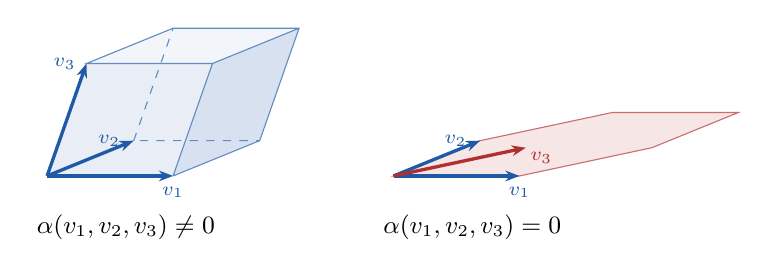
\begin{tikzpicture}[>={Stealth[length=1.8mm]},x={(1cm,0cm)},y={(0.5cm,0.32cm)},z={(0cm,1cm)}]
% left: v1=(1.6,0,0), v2=(0.4,1.4,0), v3=(0.3,0.4,1.3): independent
\begin{scope}
\coordinate (O) at (0,0,0); \coordinate (A) at (1.6,0,0); \coordinate (B) at (0.4,1.4,0); \coordinate (C) at (0.3,0.4,1.3);
\coordinate (AB) at (2.0,1.4,0); \coordinate (AC) at (1.9,0.4,1.3); \coordinate (BC) at (0.7,1.8,1.3); \coordinate (ABC) at (2.3,1.8,1.3);
\fill[figB!10] (O)--(A)--(AC)--(C)--cycle; \fill[figB!18] (A)--(AB)--(ABC)--(AC)--cycle; \fill[figB!6] (C)--(AC)--(ABC)--(BC)--cycle;
\draw[figB!70,thin] (A)--(AB)--(ABC)--(BC)--(C)--(AC)--(A) (AC)--(ABC);
\draw[figB!70,thin,dashed] (O)--(B)--(AB) (B)--(BC);
\draw[->,very thick,figB] (O)--(A) node[below,font=\scriptsize]{$v_1$};
\draw[->,very thick,figB] (O)--(B) node[left,font=\scriptsize,xshift=-1pt]{$v_2$};
\draw[->,very thick,figB] (O)--(C) node[left,font=\scriptsize]{$v_3$};
\node[font=\small] at (1.0,0,-0.65) {$\alpha(v_1,v_2,v_3)\ne0$};
\end{scope}
% right: v3 = 0.5 v1 + 0.8 v2 = (1.12,1.12,0) lies in span(v1,v2)
\begin{scope}[xshift=4.4cm]
\coordinate (O) at (0,0,0); \coordinate (A) at (1.6,0,0); \coordinate (B) at (0.4,1.4,0); \coordinate (C) at (1.12,1.12,0);
\coordinate (AB) at (2.0,1.4,0); \coordinate (AC) at (2.72,1.12,0); \coordinate (BC) at (1.52,2.52,0); \coordinate (ABC) at (3.12,2.52,0);
\fill[figR!12] (O)--(A)--(AC)--(ABC)--(BC)--(B)--cycle;
\draw[figR!70,thin] (O)--(A)--(AC)--(ABC)--(BC)--(B)--cycle;
\draw[->,very thick,figB] (O)--(A) node[below,font=\scriptsize]{$v_1$};
\draw[->,very thick,figB] (O)--(B) node[left,font=\scriptsize,xshift=-1pt]{$v_2$};
\draw[->,very thick,figR] (O)--(C) node[below right,font=\scriptsize,inner sep=1pt]{$v_3$};
\node[font=\small] at (1.0,0,-0.65) {$\alpha(v_1,v_2,v_3)=0$};
\end{scope}
\end{tikzpicture}\end{document}
